\documentclass{article}
% translate with >> pdflatex -shell-escape <file>

% This file is an extract of the PGFPLOTS manual, copyright by Christian Feuersaenger.
% 
% Feel free to use it as long as you cite the pgfplots manual properly.
%
% See
%   http://pgfplots.sourceforge.net/pgfplots.pdf
% for the complete manual.
%
% Any required input files (for <plot table> or <plot file> or the table package) can be downloaded
% at
% http://www.ctan.org/tex-archive/graphics/pgf/contrib/pgfplots/doc/latex/
% and
% http://www.ctan.org/tex-archive/graphics/pgf/contrib/pgfplots/doc/latex/plotdata/

\usepackage{pgfplots}
\pgfplotsset{compat=newest}

\pagestyle{empty}

\begin{document}
\pgfplotsset{
	small,
	title=Trimmed bounding boxes
}
\begin{center}
\begin{tabular}{rl}
	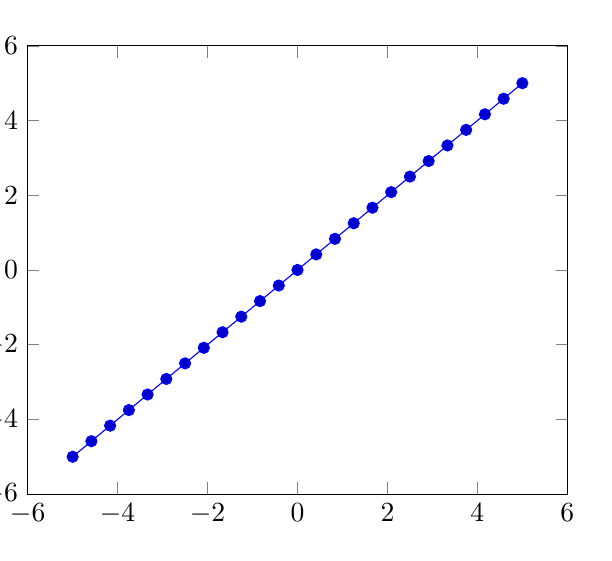
\begin{tikzpicture}[baseline,trim axis left]
		\begin{axis}
			\addplot {x};
		\end{axis}
	\end{tikzpicture}
	&
	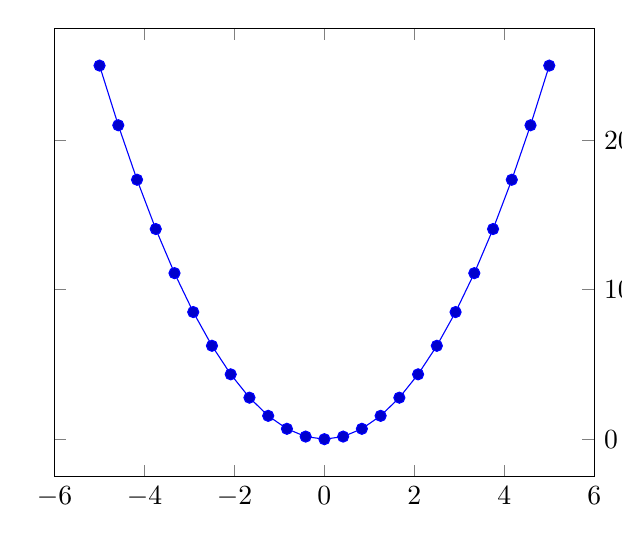
\begin{tikzpicture}[baseline,trim axis right]
	\begin{axis}[
		ylabel={$f(x)=x^2$},
		yticklabel pos=right,
		ylabel style={font=\Huge}]
		\addplot {x^2};
	\end{axis}
	\end{tikzpicture}
	\\
	%
	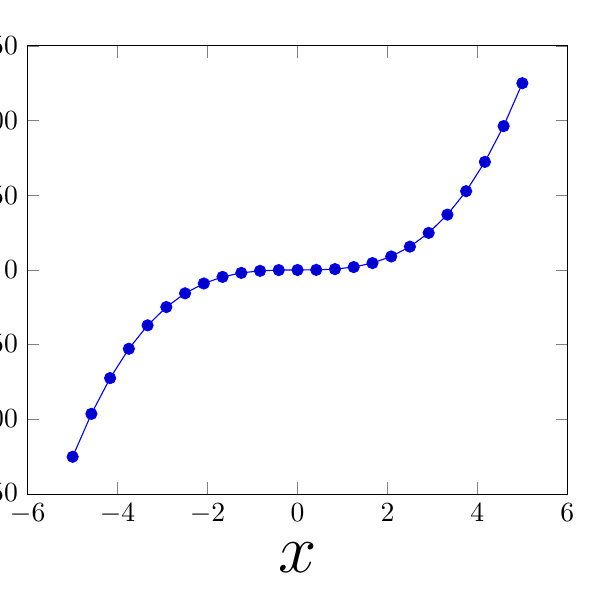
\begin{tikzpicture}[baseline,trim axis left]
	\begin{axis}[xlabel=$x$,xlabel style={font=\Huge}]
		\addplot {x^3};
	\end{axis}
	\end{tikzpicture}%
	&
	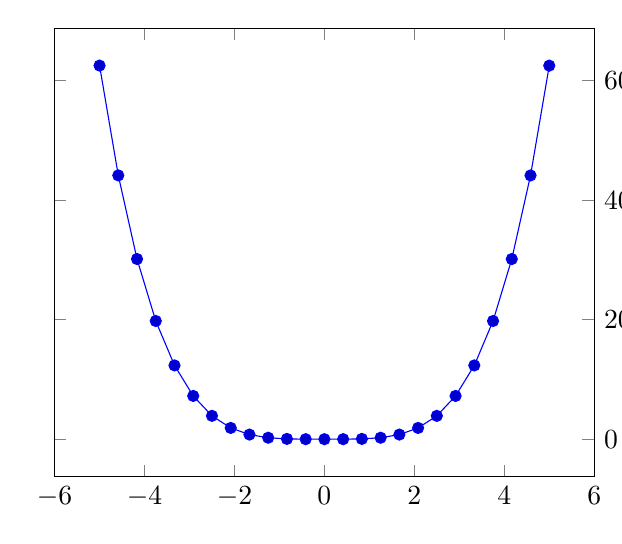
\begin{tikzpicture}[baseline,trim axis right]
	\begin{axis}[yticklabel pos=right]
		\addplot {x^4};
	\end{axis}
	\end{tikzpicture}%
	\\
\end{tabular}%
\end{center}
\end{document}
